% Section: Results
\section{Results}
\label{sec:results}

Table~\ref{tab:policy_summary} summarises the five-policy evaluation over
$n{=}300$ matched episodes.

\subsection{POMCP Exceeds the Oracle-Heuristic Ceiling}
\label{sec:results_pomcp}
POMCP was evaluated over the same $n{=}300$ episode indices as the heuristic
policies, sharing identical environment seeds, hidden courtesy types, and
observation noise; paired tests are therefore valid.
The POMCP policy achieves the lowest collision rate of all five policies:
5.0\% (95\% CI [2.7\%, 7.7\%]) and highest mean reward 57.36
([57.09, 57.63]).
After Holm--Bonferroni correction across all twenty pairwise collision and
reward comparisons ($\binom{5}{2}{\times}2$), all POMCP comparisons remain
significant.
Against the oracle-heuristic baseline, POMCP reduces collision rate from
10.3\% to 5.0\%, a 5.3\,pp absolute reduction and 51.6\% relative reduction
(McNemar $\chi^2{=}8.65$, $p_\text{adj}{=}0.014$, $|h|{=}0.204$;
discordant pairs: 5 POMCP-only vs.\ 21 oracle-only collisions,
Table~\ref{tab:mcnemar_discordants}), and increases mean reward by 0.90 points (paired
$t(299){=}3.82$, $p_\text{adj}{=}0.0011$, $d{=}0.221$).
Against the belief and rule baselines the margins are larger:
$|h|{=}0.344$, $d{=}0.316$ and $|h|{=}0.434$, $d{=}0.362$ respectively
($p_\text{adj}{<}0.001$ for both metrics in both comparisons).
Within this heuristic comparison, POMCP's reward margin over the
oracle-heuristic baseline ($d{=}0.221$) is comparable to the
oracle-heuristic margin over rule ($d{=}0.233$), indicating that UCT planning
captures safety-relevant action sequences not represented by the V-shaped
heuristic table.

\subsection{Oracle-Heuristic vs.\ Rule: Hidden Courtesy Is Decision-Relevant}
\label{sec:results_oracle}
Oracle-heuristic access to the true hidden courtesy type significantly
reduces the collision rate relative to the rule baseline:
10.3\% vs.\ 18.3\%
(McNemar $\chi^2{=}11.02$, $p_\text{adj}{=}0.005$, $|h|{=}0.230$),
and improves mean reward:
56.46 vs.\ 54.90
(paired $t(299){=}4.03$, $p_\text{adj}{=}0.00056$, $d{=}0.233$).
By-courtesy subgroup analysis (Table~\ref{tab:sig_by_courtesy}) shows that
the reward advantage is significant only in non-cooperative episodes
($p_\text{adj}{=}0.035$, $d{=}0.253$, $n{=}150$ pairs; within-subgroup exploratory, 4-test family), consistent with
the intuition that cooperative vehicles create large gaps in which the
uniform-prior heuristic already behaves well.
\textbf{This gap reflects perfect courtesy knowledge \emph{within the heuristic
action table only}; it is not the value of information for an optimal POMDP
policy, as the POMCP results in \S\ref{sec:results_pomcp} demonstrate.}

\subsection[Belief vs.\ Rule: Online Inference Is Underpowered at n=300]{Belief vs.\ Rule: Online Inference Is Underpowered at $n{=}300$}
\label{sec:results_belief}
The belief policy (collision 15.0\%, reward 55.33) is ordered between the
oracle-heuristic and rule baselines, but \textbf{neither collision rate nor
reward differences are significant after Holm--Bonferroni correction}
($p_\text{adj}{=}0.33$ for both; $d{=}0.069$, $|h|{=}0.090$).
A post-hoc power analysis shows that detecting a 3.3-percentage-point
collision-rate difference at 80\% power requires $n{\approx}1{,}960$
episodes per policy; achieved power is 19.5\%.
Given the observed effect size ($|h|{=}0.090$, $d{=}0.069$), this comparison
is underpowered and should be treated as suggestive rather than conclusive; a
confirmatory replication at $n{\geq}1{,}960$ episodes per policy is required
to support a definitive claim in either direction.

\subsection{Early-Window Convergence: The Upstream Bottleneck}
\label{sec:results_bottleneck}
Belief accuracy in the first five interaction-window steps is only 71.3\%,
rising to 90.3\% at steps 21 and beyond (Table~\ref{tab:where_when};
Figure~\ref{fig:belief_conv}).
The initial dip (step 1: 75.3\%, step 2: 71.3\%, step 3: 70.0\%) reflects
a transient in which the non-cooperative vehicle's IDM controller briefly
decelerates in response to ego detection, producing acceleration signals
that temporarily resemble cooperative behaviour.
A belief-gain sweep across five sensitivity values ($g{=}0.05$--$0.50$,
a $10{\times}$ range) shows that belief-policy collision rate is flat at
15.0\% and reward at 55.33 across every gain value
($p_\text{adj}{=}1.0$ at all gains within the five-gain Holm--Bonferroni family; Table~\ref{tab:gain_sweep};
Figure~\ref{fig:gain_sweep}).
The oracle, by contrast, improves monotonically with higher gain ($-8.0$
percentage points collision, $+1.76$ reward across the sweep).
The bottleneck lies upstream in observation quality, not downstream in the
action mapping: amplifying belief sensitivity cannot help when the
early-window belief is itself unreliable.
Replaying stored per-step rewards under close-call penalty weights
$w\in\{0.10,0.25,0.50,1.00\}$ preserves the same reward ordering
POMCP $>$ oracle $>$ belief $>$ rule $\gg$ random
(Table~\ref{tab:penalty_ablation}), so the headline ranking is not an
artifact of the manually chosen $w{=}0.25$ coefficient.
A POMCP rollout-isolation run replacing the conservative rollout trigger
($d{<}15$\,m or TTC\,$<$\,6\,s) with the heuristic emergency trigger
($d{<}8$\,m or TTC\,$<$\,3\,s) preserves the same collision rate and reward
(Table~\ref{tab:pomcp_rollout_ablation}), reducing the concern that the
POMCP result is only a rollout-conservatism artifact.
Therefore, the POMCP result should be interpreted as evidence that online
planning improves over the released heuristic action table, not as a clean
attribution to belief-state optimality alone.
Random actions provide an unconditional lower bound:
87.0\% collision rate ($|h|{=}1.52$, $p_\text{adj}{<}0.001$ vs.\ rule).
A QMDP approximation (16-state discretisation, $n{=}50$ training
episodes) was also prototyped; it achieved a 34--35\% collision rate with
50\% Q-table state coverage and is excluded from the primary comparison.
This failure is best interpreted as coverage collapse in a naive tabular
offline approximation: unvisited bins retain effectively random action values,
so the result should not be read as evidence against QMDP itself.
It motivates richer state representations, function approximation, or online
planning for future benchmark users.
Table~\ref{tab:robustness_summary} summarises the robustness and diagnostic
checks that support this interpretation.

% Table 7: Policy summary with 95% CI
% Source: eval_final_v6_cleanobs/policy_summary.csv
\begin{table}[htbp]
\centering
\caption{Policy evaluation results over $n{=}300$ matched episodes per policy.
  95\% CIs use bootstrap for binary metrics and normal approximation for
  continuous metrics.
  Collision rate ordering (lower is better):
  pomcp $<$ oracle $<$ belief $<$ rule $\ll$ random.
  Reward ordering (higher is better):
  pomcp $>$ oracle $>$ belief $>$ rule $\gg$ random.
  POMCP uses the same external Bayesian belief as \texttt{belief\_policy};
  100 UCT simulations per step.}
\label{tab:policy_summary}
\small
\resizebox{\textwidth}{!}{%
\begin{tabular}{lccccc}
\toprule
\textbf{Policy}
  & \textbf{Collision [\%]}
  & \textbf{Success [\%]}
  & \textbf{Mean Reward}
  & \textbf{Mean min TTC [s]}
  & \textbf{Close-call [\%]} \\
\midrule
pomcp\_policy
  & \textbf{5.0} [2.7,\;7.7]
  & \textbf{95.0} [92.3,\;97.3]
  & \textbf{57.36} [57.09,\;57.63]
  & 3.14 [2.61,\;3.67]
  & 11.7 \\
oracle\_policy
  & 10.3 [7.0,\;14.0]
  & 89.7 [86.0,\;93.0]
  & 56.46 [55.97,\;56.95]
  & 3.03 [2.66,\;3.39]
  & 12.0 \\
belief\_policy
  & 15.0 [11.0,\;19.0]
  & 85.0 [81.0,\;89.0]
  & 55.33 [54.59,\;56.07]
  & 2.95 [2.60,\;3.30]
  & 12.1 \\
rule\_policy
  & 18.3 [14.3,\;23.0]
  & 81.7 [77.0,\;85.7]
  & 54.90 [54.12,\;55.68]
  & 3.02 [2.66,\;3.38]
  & 11.9 \\
random\_policy
  & 87.0 [83.0,\;91.0]
  & 13.0 [\phantom{0}9.0,\;17.0]
  & 36.71 [35.31,\;38.10]
  & 1.88 [1.64,\;2.11]
  & 20.7 \\
\bottomrule
\end{tabular}}
\end{table}

% Table: Pooled significance tests (20-test joint Holm-Bonferroni)
% Family: all C(5,2)x2 = 20 pairwise comparisons applied jointly
\begin{table}[htbp]
\centering
\caption{Pooled paired hypothesis tests ($n{=}300$ pairs).
  Holm--Bonferroni correction applied jointly across all
  $\binom{5}{2}{\times}2{=}20$ comparisons.
  McNemar test for collision (binary); paired $t$-test for reward.
  Cohen's $d$ uses paired-difference SD; Cohen's $h$ uses arcsine transform;
  McNemar discordant counts are reported in Table~\ref{tab:mcnemar_discordants}.}
\label{tab:sig_pooled}
\small
\resizebox{\textwidth}{!}{%
\begin{tabular}{llcccc}
\toprule
\textbf{Comparison} & \textbf{Metric} & $p_\text{raw}$ & $p_\text{adj}$ & \textbf{Effect size} & \textbf{Sig.} \\
\midrule
\multicolumn{6}{l}{\textit{POMCP vs.\ heuristic baselines}} \\
pomcp vs oracle & Collision & 0.0033 & 0.014  & $|h|{=}0.204$ & \textbf{Yes} \\
pomcp vs oracle & Reward    & 0.0002 & 0.0011 & $d{=}0.221$   & \textbf{Yes} \\
pomcp vs belief & Collision & $<$0.001 & $<$0.001 & $|h|{=}0.344$ & \textbf{Yes} \\
pomcp vs belief & Reward    & $<$0.001 & $<$0.001 & $d{=}0.316$   & \textbf{Yes} \\
pomcp vs rule   & Collision & $<$0.001 & $<$0.001 & $|h|{=}0.434$ & \textbf{Yes} \\
pomcp vs rule   & Reward    & $<$0.001 & $<$0.001 & $d{=}0.362$   & \textbf{Yes} \\
\addlinespace
\multicolumn{6}{l}{\textit{Oracle, belief, and rule comparisons}} \\
oracle vs rule  & Collision & 0.0009 & 0.005  & $|h|{=}0.230$ & \textbf{Yes} \\
oracle vs rule  & Reward    & 0.0001 & 0.00056& $d{=}0.233$   & \textbf{Yes} \\
oracle vs belief & Collision & 0.0500 & 0.150  & $|h|{=}0.141$ & No \\
oracle vs belief & Reward   & 0.0027 & 0.014  & $d{=}0.175$   & \textbf{Yes} \\
belief vs rule  & Collision & 0.1649 & 0.330  & $|h|{=}0.090$ & No \\
belief vs rule  & Reward    & 0.2354 & 0.330  & $d{=}0.069$   & No \\
\addlinespace
\multicolumn{6}{l}{\textit{Random policy (unconditional lower bound)}} \\
rule vs random  & Collision & $<$0.001 & $<$0.001 & $|h|{=}1.519$ & \textbf{Yes} \\
rule vs random  & Reward    & $<$0.001 & $<$0.001 & $d{=}1.370$   & \textbf{Yes} \\
\bottomrule
\end{tabular}}
\begin{tablenotes}
\small
\item Remaining six comparisons (pomcp, oracle, belief, belief vs random)
  all achieve $p_\text{adj}{<}0.001$ and are omitted for brevity.
\end{tablenotes}
\end{table}

% Table: Discordant-pair counts for McNemar collision tests
% Source: eval_final_v6_cleanobs/policy_episodes.csv and pomcp_300ep_100sims/policy_episodes.csv
\begin{table}[htbp]
\centering
\caption{Discordant-pair counts underlying the paired McNemar collision tests
  in Table~\ref{tab:sig_pooled}. ``First-only'' means the first-named policy
  collided while the second did not; ``second-only'' means the reverse.}
\label{tab:mcnemar_discordants}
\small
\begin{tabular}{lrrrrc}
\toprule
\textbf{Comparison} & \textbf{First-only} & \textbf{Second-only} &
\textbf{Both} & \textbf{Neither} & $p_\text{adj}$ \\
\midrule
pomcp vs oracle & 5 & 21 & 10 & 264 & 0.014 \\
pomcp vs belief & 6 & 36 & 9 & 249 & $<0.001$ \\
pomcp vs rule & 7 & 47 & 8 & 238 & $<0.001$ \\
oracle vs rule & 12 & 36 & 19 & 233 & 0.005 \\
oracle vs belief & 15 & 29 & 16 & 240 & 0.150 \\
belief vs rule & 16 & 26 & 29 & 229 & 0.330 \\
rule vs random & 4 & 210 & 51 & 35 & $<0.001$ \\
\bottomrule
\end{tabular}
\begin{tablenotes}
\small
\item Counts sum to $n{=}300$ matched episodes for each comparison.
  Holm--Bonferroni adjusted $p$ values use the same 20-comparison family as
  Table~\ref{tab:sig_pooled}.
\end{tablenotes}
\end{table}

% Table 9: By-courtesy subgroup significance tests
% Source: eval_final_v6_cleanobs/policy_summary.json significance_tests_by_courtesy
\begin{table}[htbp]
\centering
\caption{Subgroup significance tests stratified by hidden courtesy
  ($n{=}150$ pairs per subgroup).
  Holm--Bonferroni correction applied \emph{within} each subgroup over
  4 tests (oracle vs.\ rule and belief vs.\ rule $\times$ 2 metrics);
  this is a separate, smaller family from the main 20-test analysis and
  should be interpreted as exploratory.
  The oracle reward advantage is significant only in the non-cooperative
  subgroup, consistent with hidden courtesy being most actionable
  when the merge vehicle is assertive.}
\label{tab:sig_by_courtesy}
\small
\begin{tabular}{llccccc}
\toprule
\textbf{Subgroup} & \textbf{Comparison} & \textbf{Metric} & $p_\text{adj}$ & \textbf{Effect} & \textbf{Sig.} \\
\midrule
Non-coop & oracle vs rule & Reward & 0.0348 & $d=0.253$ & \textbf{Yes} \\
Non-coop & oracle vs rule & Collision & 0.4983 & $h=-0.222$ & No \\
Non-coop & belief vs rule & Reward & 0.4058 & $d=0.185$ & No \\
Non-coop & belief vs rule & Collision & 0.6370 & $h=-0.185$ & No \\
\addlinespace
Coop & oracle vs rule & Reward & 0.0907 & $d=0.222$ & No \\
Coop & oracle vs rule & Collision & 0.1682 & $h=-0.253$ & No \\
Coop & belief vs rule & Reward & 1.0000 & $d=-0.009$ & No \\
Coop & belief vs rule & Collision & 1.0000 & $h=+0.019$ & No \\
\bottomrule
\end{tabular}
\begin{tablenotes}
\small
\item Signed $h$: positive means the first-named policy has a higher binary
  event rate for that metric; negative means it has a lower rate.
\end{tablenotes}
\end{table}

% Table 10: Belief accuracy by policy
% Source: eval_final_v6_cleanobs/policy_summary.json belief_accuracy
\begin{table}[htbp]
\centering
\caption{Bayesian belief accuracy measured on in-window steps during the
  policy evaluation (eval\_final\_v6\_cleanobs).
  Accuracy = fraction of steps where $\arg\max_m b_t(m)$ matches the true
  hidden courtesy type. For \texttt{oracle\_policy}, this diagnostic reports
  the shared external Bayesian filter run for analysis, not the one-hot
  courtesy belief passed to the oracle action table.}
\label{tab:belief_accuracy}
\small
\begin{tabular}{lcccc}
\toprule
\textbf{Policy} & \textbf{Coop acc.} & \textbf{Non-coop acc.} & \textbf{Overall acc.} & \textbf{Steps} \\
\midrule
oracle\_policy & 97.4\% & 78.4\% & 80.9\% & 4{,}386 \\
belief\_policy & 98.7\% & 79.4\% & 82.7\% & 4{,}583 \\
rule\_policy   & 97.5\% & 79.6\% & 82.6\% & 4{,}572 \\
random\_policy & 98.5\% & 81.6\% & 88.2\% & 3{,}369 \\
\bottomrule
\end{tabular}
\end{table}

% Table 11: Power analysis
% Source: review_analyses_cleanobs/corrected_power_analysis.csv
\begin{table}[htbp]
\centering
\caption{Post-hoc power analysis for collision-rate comparisons
  (two-sided pairwise Cohen's $h$, $\alpha{=}0.05$).
  The achieved $n{=}300$ is adequate for the oracle vs.\ rule gap (8.0\,pp)
  but insufficient for the smaller belief vs.\ rule gap ($\approx$3.3\,pp).}
\label{tab:power}
\small
\resizebox{\textwidth}{!}{%
\begin{tabular}{lccccc}
\toprule
\textbf{Comparison} & \textbf{Collision rates} & \textbf{$|h|$} &
\textbf{Power @ $n{=}300$} & \textbf{$n$ for 80\%} & \textbf{$n$ for 90\%} \\
\midrule
oracle vs random & 10.3\% vs.\ 87.0\% & 1.749 & $>$99.9\% & 6 & 7 \\
random vs rule & 87.0\% vs.\ 18.3\% & 1.519 & $>$99.9\% & 7 & 10 \\
oracle vs rule & 10.3\% vs.\ 18.3\% & 0.230 & 80.6\% & 296 & 396 \\
oracle vs belief & 10.3\% vs.\ 15.0\% & 0.141 & 40.7\% & 792 & 1{,}060 \\
belief vs rule & 15.0\% vs.\ 18.3\% & 0.090 & 19.5\% & 1{,}958 & 2{,}621 \\
\bottomrule
\end{tabular}}
\begin{tablenotes}
\small
\item Required $n$ is per policy. Estimates use each pair's observed
  collision rates and Cohen's $h$; no pooled collision rate across unrelated
  policies is used. These are approximate marginal-rate planning estimates;
  the paired McNemar tests themselves use the matched discordant counts in
  Table~\ref{tab:mcnemar_discordants}.
\end{tablenotes}
\end{table}

% Table: Belief accuracy by interaction step (where/when diagnostic)
% Source: D:\MERGE\where_when_cleanobs\
\begin{table}[htbp]
\centering
\caption{Belief classification accuracy as a function of interaction-window step
  number, non-cooperative episodes only (\texttt{belief\_policy},
  $n{=}300$ evaluation).
  Steps are numbered from first entry into the interaction window ($d{<}40$\,m).
  Accuracy rises as the observation sequence accumulates evidence; the
  critical early-window deficit (steps~1--5: 71.3\%) is the primary
  bottleneck for the belief policy. Brackets report bootstrap 95\% CIs for
  step-level accuracy.}
\label{tab:where_when}
\small
\begin{tabular}{lccc}
\toprule
\textbf{Interaction-window step(s)} & \textbf{Steps} &
\textbf{Episodes} & \textbf{Belief accuracy (95\% CI)} \\
\midrule
Step 1  & 150 & 150 & 75.3\% [68.7, 82.7] \\
Step 2  & 150 & 150 & 71.3\% [64.0, 78.7] \\
Step 3  & 150 & 150 & 70.0\% [62.7, 77.3] \\
Steps 4--5 & 300 & 150 & 70.0\% [65.0, 75.0] \\
Steps 6--10 & 750 & 150 & 72.5\% [69.3, 75.6] \\
Steps 11--20 & 1{,}459 & 150 & 80.7\% [78.8, 82.8] \\
Steps 21+ & 854 & 124 & 90.3\% [88.4, 92.2] \\
\midrule
All in-window steps (dataset, belief policy) & 46{,}896 & 3{,}000 & 83.6\% \\
Final step per episode (dataset)              & 3{,}000 & 3{,}000 & 93.8\% \\
\bottomrule
\end{tabular}
\end{table}

% Table: Belief-gain sweep
% Source: belief_gain_sweep/belief_gain_sweep_summary.csv
\begin{table}[htbp]
\centering
\caption{Belief-gain sweep: collision rate (\%) and mean reward vs.\ the
  belief-gain coefficient $g$ across $n{=}300$ matched episodes.
  The gain controls the V-shaped action slope
  ($p_\text{SLOWER}{=}0.735+g\cdot|2b_\text{coop}{-}1|$).
  The canonical gain (bold) is the setting used throughout the evaluation.
  Rule baseline is 18.3\% collision and 54.90 reward (constant by construction).}
\label{tab:gain_sweep}
\small
\begin{tabular}{ccccc}
\toprule
\multirow{2}{*}{\textbf{Gain $g$}} &
\multicolumn{2}{c}{\textbf{Oracle}} &
\multicolumn{2}{c}{\textbf{Belief}} \\
\cmidrule(lr){2-3}\cmidrule(lr){4-5}
& Collision (\%) & Mean reward & Collision (\%) & Mean reward \\
\midrule
0.05  & 13.7 & 55.51 & 15.0 & 55.33 \\
0.10  & 11.7 & 55.96 & 15.0 & 55.33 \\
\textbf{0.185} & \textbf{10.3} & \textbf{56.46} & \textbf{15.0} & \textbf{55.33} \\
0.30  &  8.7 & 56.83 & 15.0 & 55.33 \\
0.50  &  5.7 & 57.27 & 15.0 & 55.33 \\
\bottomrule
\end{tabular}
\begin{tablenotes}
\small
\item Belief vs.\ rule: $|h|{=}0.090$, $p_\text{adj}{=}1.0$ at every tested
  gain (McNemar, Holm--Bonferroni corrected). Oracle vs.\ rule at canonical
  gain: $|h|{=}0.230$, $p_\text{adj}{=}0.013$ after correction over the
  five-gain sweep family; the same raw test gives $p_\text{adj}{=}0.005$
  under the twenty-comparison pooled policy-evaluation family in
  Table~\ref{tab:sig_pooled}.
\end{tablenotes}
\end{table}

% Table: Close-call penalty sensitivity
% Source: eval_final_v6_cleanobs/policy_steps.csv and pomcp_300ep_100sims/policy_steps.csv
% Reward replayed as R_t = env_reward_t - w * close_call_t; no re-simulation.
\begin{table}[htbp]
\centering
\caption{Sensitivity of mean episode reward to the close-call penalty weight $w$,
  computed by replaying stored per-step columns (no re-simulation).
  Collision rates are invariant to $w$ (determined by policy actions, not the reward
  formula): POMCP 5.0\%, oracle 10.3\%, belief 15.0\%, rule 18.3\%, random 87.0\%.
  The canonical weight $w{=}0.25$ (bold column) is used throughout the primary
  evaluation.}
\label{tab:penalty_ablation}
\small
\begin{tabular}{lcccc}
\toprule
\textbf{Policy}
  & \textbf{$w{=}0.10$}
  & \textbf{$w{=}0.25$}
  & \textbf{$w{=}0.50$}
  & \textbf{$w{=}1.00$} \\
\midrule
POMCP  & 58.40 & \textbf{57.36} & 55.62 & 52.14 \\
Oracle & 57.54 & \textbf{56.46} & 54.68 & 51.10 \\
Belief & 56.40 & \textbf{55.33} & 53.54 & 49.96 \\
Rule   & 55.95 & \textbf{54.90} & 53.14 & 49.64 \\
Random & 37.93 & \textbf{36.71} & 34.67 & 30.61 \\
\bottomrule
\end{tabular}
\begin{tablenotes}
\small
\item The ordering POMCP $>$ oracle $>$ belief $>$ rule $\gg$ random is preserved
  at all four weights; the headline ranking is not an artefact of the manually
  chosen $w{=}0.25$ coefficient.
\end{tablenotes}
\end{table}

% Table: POMCP rollout isolation
% Source: pomcp_300ep_100sims and pomcp_heuristic_rollout_300ep
\begin{table}[htbp]
\centering
\caption{POMCP rollout isolation over the same $n{=}300$ matched episodes.
  The primary POMCP run uses a conservative rollout trigger
  ($d{<}15$\,m or TTC\,$<$\,6\,s). The isolation run replaces this with the
  heuristic emergency trigger ($d{<}8$\,m or TTC\,$<$\,3\,s). Comparable
  performance indicates that POMCP's headline result is not explained solely
  by rollout conservatism.}
\label{tab:pomcp_rollout_ablation}
\small
\begin{tabular}{lcccc}
\toprule
\textbf{Rollout trigger} & \textbf{Collision} & \textbf{Reward} &
\textbf{Min TTC} & \textbf{Close-call rate} \\
\midrule
Conservative ($d{<}15$, TTC$<6$) & 5.0\% & 57.36 & 3.14 & 11.7\% \\
Emergency ($d{<}8$, TTC$<3$)     & 5.0\% & 57.41 & 3.15 & 11.6\% \\
\bottomrule
\end{tabular}
\end{table}

% Table: Robustness and diagnostic checks
\begin{table}[htbp]
\centering
\caption{Robustness and diagnostic checks supporting the main claims.
  The benchmark is designed to expose confounds rather than hide them:
  each check targets a specific alternative explanation for the headline
  policy ordering or the belief-policy null result.}
\label{tab:robustness_summary}
\small
\resizebox{\textwidth}{!}{%
\begin{tabular}{>{\raggedright\arraybackslash}p{0.23\textwidth}
                >{\raggedright\arraybackslash}p{0.34\textwidth}
                >{\raggedright\arraybackslash}p{0.34\textwidth}}
\toprule
\textbf{Threat or alternative explanation} & \textbf{Check} & \textbf{Outcome} \\
\midrule
Action table too insensitive to belief
  & Belief-gain sweep over $g\in\{0.05,0.10,0.185,0.30,0.50\}$
  & Belief collision remains 15.0\% and reward 55.33 at every gain;
    oracle improves from 13.7\% to 5.7\% collision (Table~\ref{tab:gain_sweep}). \\
\addlinespace
Manual close-call reward weight drives ranking
  & Replay stored per-step rewards for $w\in\{0.10,0.25,0.50,1.00\}$
  & Reward ordering is unchanged: POMCP $>$ oracle-heuristic $>$ belief $>$ rule
    $\gg$ random (Table~\ref{tab:penalty_ablation}). \\
\addlinespace
POMCP advantage is only conservative rollout bias
  & Replace POMCP rollout trigger from $d{<}15$\,m or TTC$<6$\,s to
    heuristic emergency trigger $d{<}8$\,m or TTC$<3$\,s
  & Collision remains 5.0\%; reward changes only from 57.36 to 57.41
    (Table~\ref{tab:pomcp_rollout_ablation}). \\
\addlinespace
Diagonal observation likelihood hides correlated features
  & Held-out full-covariance Gaussian over \{\emph{ard}, \emph{mvs}, \emph{mva}\}
  & Offline final-step belief accuracy improves from 92.2\% to 97.7\%;
    closed-loop full-covariance evaluation is identified as the next benchmark
    variant (Table~\ref{tab:covariance_ablation}). \\
\addlinespace
Binary significance depends only on marginal rates
  & Report paired McNemar discordant counts for collision tests
  & Key comparisons are supported by asymmetric discordants, e.g.,
    pomcp vs.\ oracle-heuristic: 5 vs.\ 21 first/second-only collisions
    (Table~\ref{tab:mcnemar_discordants}). \\
\addlinespace
Belief-vs-rule null is overinterpreted
  & Post-hoc power analysis using pairwise observed collision rates
  & Achieved power is 19.5\%; $n{\approx}1{,}960$ per policy is required for
    80\% power at the observed 3.3\,pp gap (Table~\ref{tab:power}). \\
\bottomrule
\end{tabular}}
\end{table}


\begin{figure}[htbp]
  \centering
  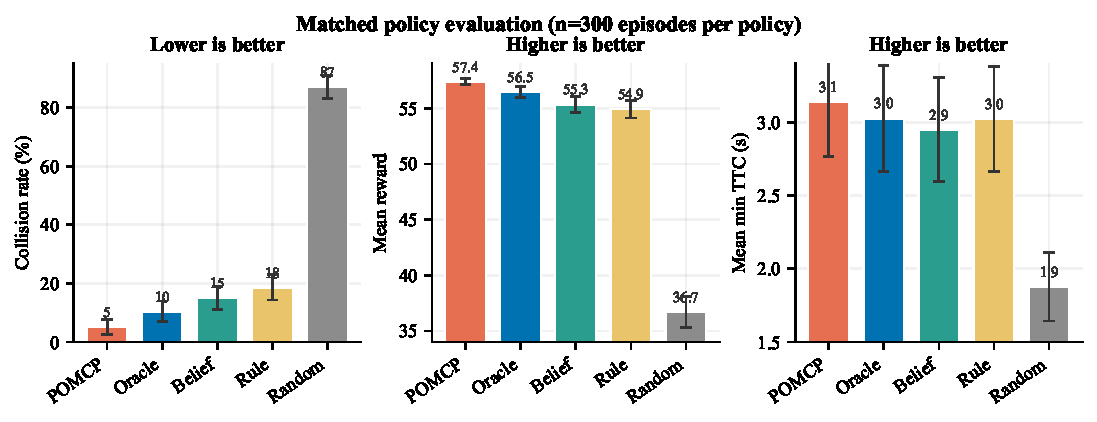
\includegraphics[width=\linewidth]{figures/policy_comparison_main_metrics}
  \caption{Policy comparison on collision rate, mean reward, and mean
    minimum TTC with 95\% CIs over $n{=}300$ matched episodes.
    POMCP achieves the best collision rate and reward; oracle-heuristic
    access significantly outperforms rule; belief is ordered between
    oracle-heuristic and rule but is not significantly better than rule at
    $n{=}300$.}
  \label{fig:policy_comparison}
\end{figure}

\begin{figure}[htbp]
  \centering
  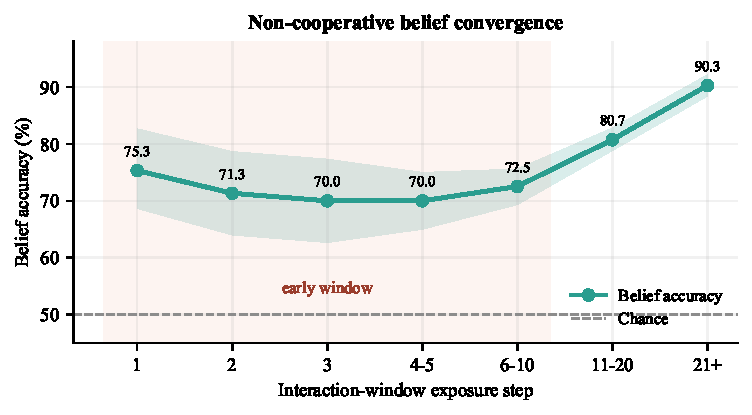
\includegraphics[width=0.7\linewidth]{figures/belief_convergence}
  \caption{Belief accuracy as a function of interaction-window step number
    for non-cooperative episodes (\texttt{belief\_policy}).
    Early-window accuracy (steps 1--5: 71.3\%) is the primary bottleneck;
    accuracy rises to 90.3\% at steps 21 and beyond.}
  \label{fig:belief_conv}
\end{figure}

\begin{figure}[htbp]
  \centering
  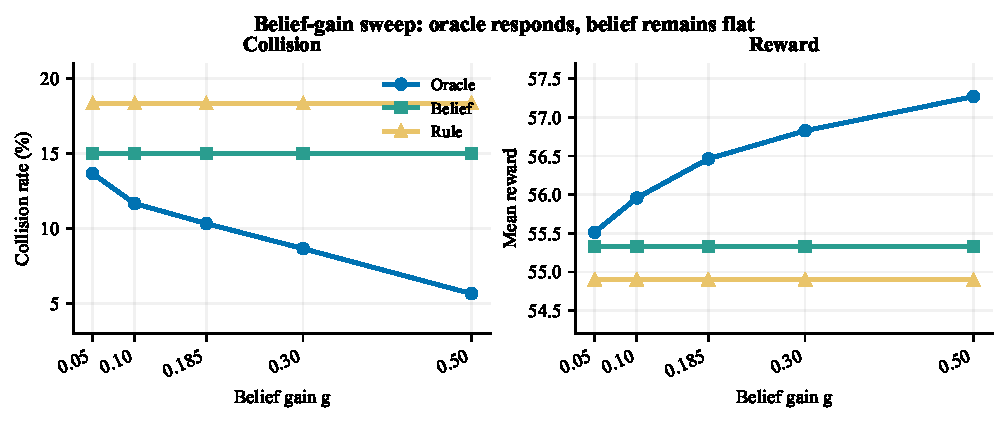
\includegraphics[width=0.85\linewidth]{figures/belief_gain_sweep}
  \caption{Belief-gain sweep over a $10{\times}$ range in action sensitivity.
    The belief policy remains flat in collision rate and reward, while the
    oracle improves as gain increases. The sweep rules out the hypothesis that
    the belief null is caused primarily by insufficient action-table gain.}
  \label{fig:gain_sweep}
\end{figure}
